\let\negmedspace\undefined
\let\negthickspace\undefined
\documentclass[journal]{IEEEtran}
\usepackage[a5paper, margin=10mm, onecolumn]{geometry}
%\usepackage{lmodern} % Ensure lmodern is loaded for pdflatex
\usepackage{tfrupee} % Include tfrupee package

\setlength{\headheight}{1cm} % Set the height of the header box
\setlength{\headsep}{0mm}     % Set the distance between the header box and the top of the text

\usepackage{gvv-book}
\usepackage{gvv}
\usepackage{cite}
\usepackage{amsmath,amssymb,amsfonts,amsthm}
\usepackage{algorithmic}
\usepackage{graphicx}
\usepackage{textcomp}
\usepackage{xcolor}
\usepackage{txfonts}
\usepackage{listings}
\usepackage{enumitem}
\usepackage{mathtools}
\usepackage{gensymb}
\usepackage{comment}
\usepackage[breaklinks=true]{hyperref}
\usepackage{tkz-euclide}
\usepackage{listings}                                     
\def\inputGnumericTable{}                                 
\usepackage[utf8]{inputenc}                                
\usepackage{color}                                            
\usepackage{array}                                            
\usepackage{longtable}                                       
\usepackage{calc}                                             
\usepackage{multirow}                                         
\usepackage{hhline}                                           
\usepackage{ifthen}                                           
\usepackage{lscape}
\renewcommand{\thefigure}{\theenumi}
\renewcommand{\thetable}{\theenumi}
\setlength{\intextsep}{10pt} % Space between text and floats

\numberwithin{equation}{enumi}
\numberwithin{figure}{enumi}
\renewcommand{\thetable}{\theenumi}

% Marks the beginning of the document
\begin{document}
\bibliographystyle{IEEEtran}

\title{Question-6.5.20}
\author{EE24BTECH11048-NITHIN.K} 
%\maketitle
%\newpage
%\bigskip
{\let\newpage\relax\maketitle}
\textbf{Question:} \\
Show that the right circular cylinder of given surface and maximum volume is such that its height is equal to the diameter of the base.

\textbf{Theoretical Solution:} \\
Total Surface Area of cylinder is
\begin{align}
	S = 2\pi rh + 2\pi r^2
\end{align}
Where r is the radius of base of cylinder and h is the height of cylinder. \\
The Volume of cylinder is
\begin{align}
	V = \pi r^2h
\end{align}
For the Given Surface Area writing h in terms of r
\begin{align}
	S = 2\pi rh + 2\pi r^2
\end{align}
\begin{align}
	h = \frac{S - 2\pi r^2}{2\pi r}
\end{align}
Expresssing Volume as a function of r
\begin{align}
	V = \pi r^2h
\end{align}
\begin{align}
	V = \frac{r\brak{S - 2\pi r^2}}{2}
\end{align}
Differentiate and Find Critical Points
Differentiate $V\brak{r}$ with respect to r
\begin{align}
	\frac{dV}{dr} = \frac{S - 6\pi r^2}{2}
\end{align}
Setting $\frac{dV}{dr} = 0$ to find the critical points:
\begin{align}
	S - 6\pi r^2 = 0
\end{align}
\begin{align}
	r = \sqrt{\frac{S}{6\pi}}
\end{align}
Substituting this r into our expression for h:
\begin{align}
	h = \frac{S - 2\pi r^2}{2\pi r}
\end{align}
\begin{align}
	h = \frac{6\pi r^2 - 2\pi r^2}{2\pi r}
\end{align}
\begin{align}
	h = 2r
\end{align}
\textbf{Computational Solution:} \\
To Maximize Volume 
\begin{align}
	V = \frac{r\brak{S - 2\pi r^2}}{2} 
\end{align}
\begin{align}
	f\brak{r} = \frac{r\brak{S - 2\pi r^2}}{2}
\end{align}
Applying Gradient Ascent
\begin{align}
	r_{n+1} = r_n + \mu f^\prime\brak{r_n}
\end{align}
where $\mu$ is the step size
\begin{align}
	f^\prime\brak{r_n} = \frac{S - 6\pi {r_n}^2}{2}
\end{align}
Difference equation is
\begin{align}
	r_{n+1} = r_n + \mu \brak{\frac{S - 6\pi {r_n}^2}{2}}
\end{align}
Using $\mu = 0.001$ and S = 1000 the radius for maximum volume is 7.283656 units theoretically And Using Gradient Ascent the radius came out to be 7.28365620 units. \\
Using Geometric Programming(cvxpy,mosek) module the value of radius is 7.283563.

\begin{figure}[H]
    \centering
    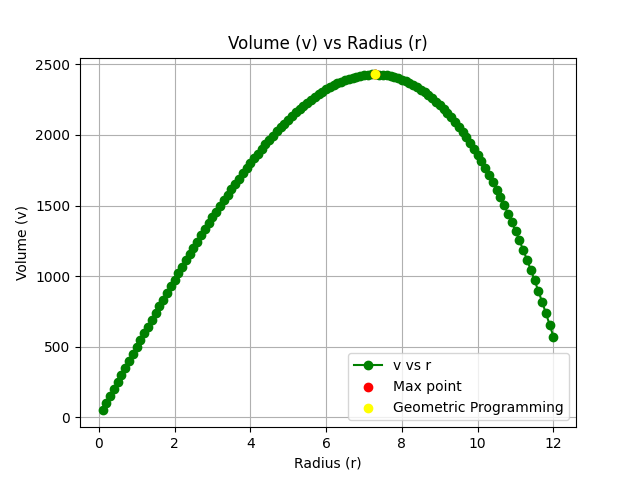
\includegraphics[width=0.8\textwidth]{figs/fig.png}
\end{figure}
\end{document}
